\documentclass[9pt]{extarticle}

\usepackage{geometry}                           % To define page size, margins, etc.
\usepackage[pdftex]{hyperref}                   % For hyper-references in the generated PDF.
\usepackage[hyperref]{xcolor}                   % To use colours in the document.
\usepackage[pdftex]{graphicx}                   % To import graphics.
\usepackage{epstopdf}                           % For on-the-fly conversion of eps to pdf.
\usepackage[british]{babel}                     % For British English hyphenation patterns.
\usepackage[latin1]{inputenc}                   % For Latin1 (ISO-8859-1) input encoding.
\usepackage[T1]{fontenc}                        % For T1 character encoding.
\usepackage{textcomp}                           % For T1 character encoding.
\usepackage{ae}                                 % For T1 encoding using Type 1 fonts.
\usepackage{mathptmx}                           % For Type 1 "Times Roman" serif text and math.
\usepackage[scaled=0.92]{helvet}                % For Type 1 "Helvetica" sans serif text.
\usepackage{courier}                            % For Type 1 "Courier" monospaced text.
\usepackage{pifont}				% For dingbat symbols.
\usepackage{xspace}                             % For automatic handling of spaces after macros.
\usepackage{multirow}				% For merging rows.
\usepackage{colortbl}
\usepackage{soul}				% For strike-through.
\usepackage[titles]{tocloft}                    % For Table of Contents customisation.
\usepackage{subfig}                             % For subfigures.
\usepackage{fancyvrb}                           % For fancy verbatim environments.
\usepackage[stable]{footmisc}                   % For stable footnotes.
\usepackage{float}                              % For extra control over floats.
\usepackage{titlesec}                           % To configure sections headings.
\usepackage[nottoc]{tocbibind}                  % To put the Bibliography in the TOC.
\usepackage{units}                              % To typeset units.

\geometry{dvipdfm,a4paper,portrait,centering,tmargin=1.5cm,bmargin=1.5cm,lmargin=2.5cm,rmargin=2.5cm,nomarginpar}

\definecolor{ins}{RGB}{0,100,0}
\definecolor{del}{RGB}{139,0,0}

\definecolor{muss}{RGB}{0,100,0}
\definecolor{darf}{RGB}{208,96,16}
\definecolor{nein}{RGB}{139,0,0}

\definecolor{rex}{rgb}{1.0,0.2,0.2}
\definecolor{no}{gray}{0.5}

\definecolor{composition}{rgb}{0,0.3,0}
\definecolor{manuscript}{rgb}{0,0,0.3}


\hypersetup{%
	linkcolor=RoyalBlue,
	urlcolor=RoyalBlue,
	plainpages=false,
	pdfpagelabels,
	hyperindex,
	colorlinks=true}

\hypersetup{%
	pdftitle={Lambtex Quick Reference},
	pdfauthor={Dario Teixeira (dario.teixeira@yahoo.com)},
	pdfsubject={lambtex},
	pdfkeywords={lambtex, lambdoc}}

\pagestyle{empty}

\begin{document}

\newcommand{\muss}[0]{\textcolor{muss}{\ding{52}}}
\newcommand{\mussz}[0]{\textcolor{muss}{\ding{52}$_{\emptyset}$}}
\newcommand{\darf}[0]{\textcolor{darf}{$\approx$}}
\newcommand{\darfz}[0]{\textcolor{darf}{$\approx_{\emptyset}$}}
\newcommand{\nein}[0]{\textcolor{nein}{\ding{56}}}
\newcommand{\neinz}[0]{\textcolor{nein}{\ding{56}$_{\emptyset}$}}
\newcommand{\dep}[0]{\nein\textbf{/}\muss}
\newcommand{\depz}[0]{\neinz\textbf{/}\mussz}
\newcommand{\no}[0]{\textcolor{no}{---}}

\newcommand{\C}[0]{\textcolor{composition}{C}}
\newcommand{\M}[0]{\textcolor{manuscript}{M}}

\newcommand{\op}[1]{\textbf{#1}}
\newcommand{\hd}[1]{\bfseries\textsc{#1}}
\newcommand{\ins}[1]{\textcolor{ins}{#1}}
\newcommand{\del}[1]{\textcolor{del}{#1}}
\newcommand{\simc}[1]{\textcolor{composition}{\texttt{\bfseries$\backslash$#1}}}
\newcommand{\simm}[1]{\textcolor{manuscript}{\texttt{\bfseries$\backslash$#1}}}
\newcommand{\envc}[1]{\textcolor{composition}{\texttt{\bfseries#1}}}
\newcommand{\envm}[1]{\textcolor{manuscript}{\texttt{\bfseries#1}}}
\newcommand{\textsubscript}[1]{\ensuremath{_{\textrm{#1}}}}

\newcommand{\param}[1]{\textsc{\{\emph{#1}\}}}
\newcommand{\inline}[0]{\param{inline}}
\newcommand{\thelabel}[0]{\param{label}}
\newcommand{\raw}[0]{\param{raw}}

\newcommand{\rexoper}[1]{\textcolor{rex}{\textbf{#1}}}
\newcommand{\rexgroup}[2]{\,\rexoper{[}#1\rexoper{]}\textsuperscript{\rexoper{#2}}\,}
\newcommand{\rexo}[1]{\rexgroup{#1}{?}}
\newcommand{\rexp}[1]{\rexgroup{#1}{+}}

\newcommand{\ex}[1]{\small\texttt{#1}}

\renewcommand{\arraystretch}{1.05}
\setlength{\arrayrulewidth}{0.6pt}

\begin{center}
\noindent{\Large\bfseries\textsc{Lambtex Quick Reference}}\\
\vspace*{0.25cm}
\noindent{\large\textsc{Dario Teixeira}}
\end{center}

\begin{center}
\small
\begin{tabular}{|r|rlllllc|}

\hline

\rule{0ex}{2.6ex} & 			&		& \multicolumn{4}{c}{\hd{Parameters}}							& \\[0.2ex]

\cline{4-7}

\rule{0ex}{2.6ex} & \hd{Command}	& \hd{Synonyms}	& \hd{Primary}			& \hd{Order}	& \hd{Label}	& \hd{Extra}		& \hd{T} \\[0.2ex]

\hline

\multirow{19}{*}{\rotatebox{90}{\hd{Inline commands}}}

& \simc{br}		& \no				& \no				& \nein		& \nein		& \neinz		& \C \rule{0ex}{2.6ex}\\
& \simc{glyph}		& \no				& \thelabel\raw			& \nein		& \nein		& \neinz		& \C \\
& \simc{bold}		& \simc{b}, \simc{strong}	& \inline			& \nein		& \nein		& \neinz		& \C \\
& \simc{emph}		& \simc{i}, \simc{em}		& \inline			& \nein		& \nein		& \neinz		& \C \\
& \simc{code}		& \simc{tt}			& \inline			& \nein		& \nein		& \neinz		& \C \\
& \simc{caps}		& \no				& \inline			& \nein		& \nein		& \neinz		& \C \\
& \simc{ins}		& \no				& \inline			& \nein		& \nein		& \neinz		& \C \\
& \simc{del}		& \no				& \inline			& \nein		& \nein		& \neinz		& \C \\
& \simc{sup}		& \no				& \inline			& \nein		& \nein		& \neinz		& \C \\
& \simc{sub}		& \no				& \inline			& \nein		& \nein		& \neinz		& \C \\
& \simc{mbox}		& \no				& \inline			& \nein		& \nein		& \neinz		& \C \\
& \simc{span}		& \no				& \inline			& \nein		& \nein		& \ex{class}		& \C \\
& \simc{link}		& \simc{a}			& \raw\rexo{\inline}		& \nein		& \nein		& \neinz		& \C \\
& \simm{cite}		& \no				& \thelabel			& \nein		& \nein		& \neinz		& \M \\
& \simm{see}		& \no				& \thelabel			& \nein		& \nein		& \neinz		& \M \\
& \simm{ref}		& \no				& \thelabel			& \nein		& \nein		& \neinz		& \M \\
& \simm{sref}		& \no				& \thelabel			& \nein		& \nein		& \neinz		& \M \\
& \simm{mref}		& \no				& \thelabel\inline		& \nein		& \nein		& \neinz		& \M \\
& \simm{\emph{macro}}	& \no				& \rexp{\inline}		& \nein		& \nein		& \neinz		& \M \\
& \simm{arg}		& \no				& \raw				& \nein		& \nein		& \neinz		& \M \\[0.2ex]

\hline

\multirow{39}{*}{\rotatebox{90}{\hd{Block commands}}}

& \simc{paragraph}	& \simc{p}			& \inline			& \nein		& \nein		& \ex{initial}, \ex{indent} & \C \rule{0ex}{2.6ex}\\
& \envc{itemize}	& \envc{ul}, \envc{itemise}	& \no				& \nein		& \nein		& \ex{bul}		& \C \\
& \envc{enumerate}	& \envc{ol}			& \no				& \nein		& \nein		& \ex{num}		& \C \\
& \envc{description}	& \envc{dl}			& \no				& \nein		& \nein		& \neinz		& \C \\
& \envc{qanda}		& \no				& \no				& \nein		& \nein		& \neinz		& \C \\
& \envc{verse}		& \no				& \no				& \nein		& \nein		& \neinz		& \C \\
& \envc{quote}		& \no				& \no				& \nein		& \nein		& \neinz		& \C \\
& \envc{mathtex}	& \no				& \no				& \nein		& \nein		& \neinz		& \C \\
& \envc{mathml}		& \no				& \no				& \nein		& \nein		& \neinz		& \C \\
& \envc{source}		& \no				& \no				& \nein		& \nein		& \ex{box}, \ex{nums}, \ex{zebra}, \ex{lang}& \C \\
& \envc{tabular}	& \no				& \raw				& \nein		& \nein		& \neinz		& \C \\
& \envc{verbatim}	& \envc{pre}			& \no				& \nein		& \nein		& \ex{mult}		& \C \\
& \simc{picture}	& \no				& \thelabel\raw			& \nein		& \nein		& \ex{frame}, \ex{width}& \C \\
& \envc{subpage}	& \no				& \no				& \nein		& \nein		& \neinz		& \C \\
& \envm{decor}		& \no				& \no				& \nein		& \nein		& \ex{float}		& \M \\
& \envm{pull}		& \no				& \rexo{\inline}		& \nein		& \nein		& \ex{float}		& \M \\
& \envm{\emph{boxout}}	& \no				& \rexo{\inline}		& \depz		& \nein		& \ex{float}		& \M \\
& \envm{\emph{theorem}}	& \no				& \rexo{\inline}		& \depz		& \nein		& \ex{float}		& \M \\
& \envm{equation}	& \no				& \rexo{\inline}		& \dep		& \darf		& \ex{float}		& \M \\
& \envm{printout}	& \no				& \rexo{\inline}		& \dep		& \darf		& \ex{float}		& \M \\
& \envm{table}		& \no				& \rexo{\inline}		& \dep		& \darf		& \ex{float}		& \M \\
& \envm{figure}		& \no				& \rexo{\inline}		& \dep		& \darf		& \ex{float}		& \M \\
& \simm{part}		& \no				& \inline			& \depz		& \darf		& \neinz		& \M \\
& \simm{appendix}	& \no				& \no				& \nein		& \darf		& \neinz		& \M \\
& \simm{section}	& \simm{h1}			& \inline			& \depz		& \darf		& \neinz		& \M \\
& \simm{subsection}	& \simm{h2}			& \inline			& \depz		& \darf		& \neinz		& \M \\
& \simm{subsubsection}	& \simm{h3}			& \inline			& \depz		& \darf		& \neinz		& \M \\
& \simm{bibliography}	& \no				& \no				& \nein		& \darf		& \neinz		& \M \\
& \simm{notes}		& \no				& \no				& \nein		& \darf		& \neinz		& \M \\
& \simm{toc}		& \no				& \no				& \nein		& \darf		& \neinz		& \M \\
& \simm{title}		& \no				& \inline			& \nein		& \nein		& \neinz		& \M \\
& \simm{subtitle}	& \no				& \inline			& \nein		& \nein		& \neinz		& \M \\
& \envm{abstract}	& \no				& \no				& \nein		& \nein		& \neinz		& \M \\
& \simm{rule}		& \simm{hr}			& \no				& \nein		& \nein		& \neinz		& \M \\
& \envm{bib}		& \no				& \no				& \nein		& \darf		& \neinz		& \M \\
& \envm{note}		& \no				& \no				& \nein		& \darf		& \neinz		& \M \\
& \envm{macrodef}	& \no				& \raw\raw\inline		& \nein		& \nein		& \neinz		& \M \\
& \envm{boxoutdef}	& \no				& \raw\rexo{\inline\rexo{\raw}}	& \nein		& \nein		& \neinz		& \M \\
& \envm{theoremdef}	& \no				& \raw\inline\rexo{\raw}	& \nein		& \nein		& \neinz		& \M \\[0.2ex]

\hline

\multirow{12}{*}{\rotatebox{90}{\hd{Auxiliary commands}}}

& \simc{item}		& \simc{li}			& \no				& \nein		& \nein		& \neinz		& \C \rule{0ex}{2.6ex}\\
& \simc{item}		& \simc{li}			& \inline			& \nein		& \nein		& \neinz		& \C \\
& \simc{question}	& \no				& \rexo{\inline}		& \nein		& \nein		& \neinz		& \C \\
& \simc{rquestion}	& \no				& \no				& \nein		& \nein		& \neinz		& \C \\
& \simc{answer}		& \no				& \rexo{\inline}		& \nein		& \nein		& \neinz		& \C \\
& \simc{ranswer}	& \no				& \no				& \nein		& \nein		& \neinz		& \C \\
& \simc{head}		& \no				& \no				& \nein		& \nein		& \neinz		& \C \\
& \simc{body}		& \no				& \no				& \nein		& \nein		& \neinz		& \C \\
& \simc{foot}		& \no				& \no				& \nein		& \nein		& \neinz		& \C \\
& \simm{who}		& \no				& \inline			& \nein		& \nein		& \neinz		& \M \\
& \simm{what}		& \no				& \inline			& \nein		& \nein		& \neinz		& \M \\
& \simm{where}		& \no				& \inline			& \nein		& \nein		& \neinz		& \M \\[0.2ex]
 
\hline

\end{tabular}
\end{center}

\clearpage

\begin{center}
\centering
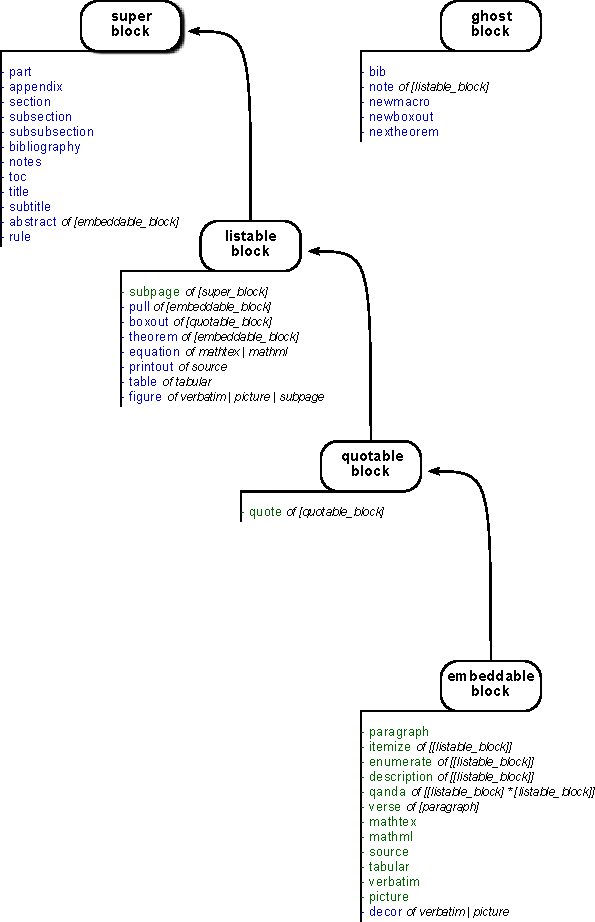
\includegraphics[height=25cm]{hierarchy.pdf}
\end{center}

\end{document}

